\tikzstyle{txt} = [text centered, inner sep=0pt]

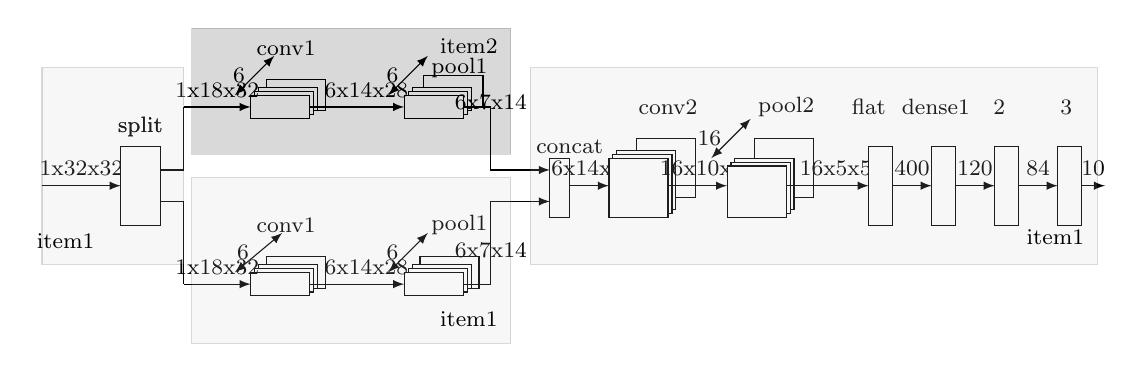
\begin{tikzpicture}[scale=1.0,
z={({0.3cm*cos(45)},{0.3cm*sin(45)})},
>=latex, 
font=\footnotesize,
]

% Big Input images



\draw[->] (-3,1.5) -- node[above] {$1$x$32$x$32$} (-2,1.5);


% SPLIT
\draw[fill=white] (-2,1) rectangle (-1.5,2);
\draw (-1.75,2.25)node[txt] (conv1){split};
\draw[-] (-1.5,1.7) -- (-1.2,1.7) -| (-1.2,2.5);
\draw[-] (-1.5,1.3) -- (-1.2,1.3) -| (-1.2,.25);


%CONV1
\draw[fill=white] (0.25+4*0.05-.6,4*0.05) rectangle (1+4*0.05-.6,.4+4*0.05);
\foreach \foreach \z in {2,...,0}  {%
 \draw[fill=white] (0.25+\z*0.05-.6,.1+\z*0.05) rectangle (1+\z*0.05-.6,.4+\z*0.05);
}
\draw (0.7-.6,1)node[txt] (conv1){conv1};
\draw[->] (-1.2,0.25) -- node[above] {$1$x$18$x$32$} (0.25-.6,0.25);
\draw[<->] (.25-0.2-.6,.4+0*0.05) -- node[left] {$6$} (.25+0.4-.6,.4+0.5);

%MAXPOOL1
\draw[fill=white] (2.5+4*0.05-.9,4*0.05) rectangle (3.25+4*0.05-.9,0.40+4*0.05);
\foreach \foreach \z in {2,...,0}  {%
 \draw[fill=white] (2.5+\z*0.05-.9,0.1+\z*0.05) rectangle (3.25+\z*0.05-.9,.40+\z*0.05);
}
\draw (3.2-.9,1)node[txt] (conv1){pool1};
\draw[->] (1-.6,0.25) -- node[above,pos=0.6] {$6$x$14$x$28$} (2.5-.9,0.25);
\draw[<->] (2.5-0.2-.9,0.4+0*0.05) -- node[left] {$6$} (2.5+0.3-.9,0.4+0.5);


\draw[fill=white] (-2,1) rectangle (-1.5,2);
\draw (-1.75,2.25)node[txt] (conv1){split};


%CONV12
\draw[fill=white] (0.25+4*0.05-.6,4*0.05+2.25) rectangle (1+4*0.05-.6,.40+4*0.05+2.25);
\foreach \foreach \z in {2,...,0}  {%
 \draw[fill=white] (0.25+\z*0.05-.6,.1+\z*0.05+2.25) rectangle (1+\z*0.05-.6,.40+\z*0.05+2.25);
}
\draw (0.7-.6,1+2.25)node[txt] (conv12){conv1};
\draw[->] (-1.2,2.5) -- node[above] {$1$x$18$x$32$} (0.25-.6,2.5);
\draw[<->] (.25-0.2-.6,.4+0*0.05+2.25) -- node[left] {$6$} (.25+0.3-.6,.4+0.5+2.25);


%MAXPOOL12
\draw[fill=white] (2.5+5*0.05-.9,5*0.05+2.25) rectangle (3.25+5*0.05-.9,0.40+5*0.05+2.25);
\foreach \foreach \z in {2,...,0}  {%
 \draw[fill=white] (2.5+\z*0.05-.9,0.1+\z*0.05+2.25) rectangle (3.25+\z*0.05-.9,.40+\z*0.05+2.25);
}
\draw (3.2-.9,1+2)node[txt] (conv12){pool1};
\draw[->] (1-.6,0.5+2) -- node[above,pos=0.6] {$6$x$14$x$28$} (2.5-.9,0.5+2);
\draw[<->] (2.5-0.2-.9,0.4+0*0.05+2.25) -- node[left] {$6$} (2.5+0.3-.9,0.4+0.5+2.25);

%CONCAT
\draw[fill=white] (4.75-1.3,1.1) rectangle (5.0-1.3,1.85);
\draw (4.80-1.1,2)node[txt] (concat){concat};
\draw[->] (3.25-.9,0.25) -| node[above,pos=0.6] {$6$x$7$x$14$} (4-1.3,0.5+.8) -- (4.75-1.3,0.5+.8);
\draw[->] (3.25-.9,2.5) -| node[above,pos=0.6] {$6$x$7$x$14$} (4-1.3,0.5+1.2) -- (4.75-1.3,0.5+1.2);

%CONV2
\draw[->] (5-1.3,1.5) -- node[above,pos=0.6] {$6$x$14$x$14$} (5.5-1.3,1.5);
\draw[fill=white] (5.5+7*0.05-1.3,7*0.05+1) rectangle (6.25+7*0.05-1.3,0.75+7*0.05+1);
\draw (6.25-1.3,1.5+1)node[txt] (conv1){conv2};
% \draw[->] (3.25,2.5) -| node[above,pos=0.6] {$6$x$14$x$7$} (4,0.5+1.2) -- (4.75,0.5+1.2);
\foreach \foreach \z in {2,...,0}  {%
 \draw[fill=white] (5.5+\z*0.05-1.3,0.1+\z*0.05+1) rectangle (6.25+\z*0.05-1.3,0.85+\z*0.05+1);
}
% \draw[<->] (5.5-0.2,0.85+0*0.05+1) -- node[left] {$16$} (4.75+0.3,0.85+0.5+1);

%MAXPOOL2
\draw[fill=white] (7+7*0.05-1.3,7*0.05+1) rectangle (7.75+7*0.05-1.3,0.75+7*0.05+1);
\draw[->] (6.25-1.3,0.5+1) -- node[above,pos=0.67] {$16$x$10$x$10$} (7-1.3,0.5+1);
\foreach \foreach \z in {2,...,0}  {%
 \draw[fill=white] (7+\z*0.05-1.3,0.1+\z*0.05+1) rectangle (7.75+\z*0.05-1.3,0.75+\z*0.05+1);
}
\draw (7.75-1.3,1.5+1)node[txt] (conv1){pool2};
\draw[<->] (7-0.2-1.3,0.85+0*0.05+1) -- node[left] {$16$} (7+0.3-1.3,0.85+0.5+1);
\draw[->] (7.75-1.3,0.5+1) -- node[above,pos=0.6] {$16$x$5$x$5$} (9-1.5,0.5+1);

\draw[fill=white] (9-1.5,0+1) rectangle (9.3-1.5,1+1);
\draw[->] (9.3-1.5,0.5+1) -- node[above] {$400$} (9.8-1.5,0.5+1);
\draw (9-1.5,1.5+1)node[txt] (conv1){flat};

%dense1
\draw[fill=white] (9.8-1.5,0+1) rectangle (10.1-1.5,1+1);
%dense2
\draw[fill=white] (10.6-1.5,0+1) rectangle (10.9-1.5,1+1);
%dense3
\draw[fill=white] (11.4-1.5,0+1) rectangle (11.7-1.5,1+1);
\draw[->] (10.1-1.5,0.5+1) --node[above] {$120$}(10.6-1.5,0.5+1);
\draw[->] (10.9-1.5,0.5+1) --node[above] {$84$} (11.4-1.5,0.5+1);
\draw (10.5-1.5,1.5+1)node[txt] (conv1){dense1 \hspace{.1cm} 2 \hspace{.5cm} 3};



\draw[->] (11.7-1.5,0.5+1) -- node[above] {$10$} (12-1.5,0.5+1);



\coordinate (item1A) at (-3 ,.5);
\coordinate (item1B) at (-1.2,3);       
\draw [fill=gray!40, opacity=.15](item1A) rectangle (item1B) 
                    node[xshift=-1.5cm, yshift=-2.2cm, opacity=1] {item1};


\coordinate (item1A) at (-1.1 , -.5);
\coordinate (item1B) at (4.25-1.3,1.6);       
\draw [fill=gray!40, opacity=.15](item1A) rectangle (item1B) 
                    node[xshift=-3.5ex, yshift=-1.8cm, opacity=1] {item1};


\coordinate (item2A) at (-1.1, 1.9);
\coordinate (item2B) at (4.25-1.3,3.5); 
 \draw [fill=gray!200, opacity=.15](item2A) rectangle (item2B) 
                    node[xshift=-3.5ex, yshift=-1.5ex, opacity=1] {item2};



\coordinate (item1A) at (4.5-1.3 , 0.5);
\coordinate (item1B) at (10.4,3);       
\draw [fill=gray!40, opacity=.15](item1A) rectangle (item1B) 
                    node[xshift=-3.5ex, yshift=-2.15cm, opacity=1] {item1};

\end{tikzpicture}
